\documentclass[11pt,openright,final]{unsa}
\title{Titulo de la tesis}
\author{Nombre completo del autor de la Tesis}%
\examinerfour{Prof. Dr. Nombre Apellido}{Externo}{Universidad del ABC} % of being the case
\date{19 de Junio del 2018}
\dedicate{A Dios, por todo lo que me ha dado, a todos los profesores
por sus enseñanzas y algunos amigos.}


\usepackage{ifluatex}


\ifluatex
    \usepackage{fontspec}
    \setsansfont{CMU Sans Serif}%{Arial}
    \setmainfont{CMU Serif}%{Times New Roman}
    \setmonofont{CMU Typewriter Text}%{Consolas}
    \defaultfontfeatures{Ligatures={TeX}}
\else
    \usepackage[utf8]{inputenc}
    \usepackage[T2A,T1]{fontenc}
\fi

\usepackage[spanish]{babel}
\usepackage{algorithmic}
\usepackage[table,xcdraw]{xcolor}

\begin{document}%%%%%%%%-------------------------------------------------------
\makeFirstCover \makeSecondCover %
\begin{frontmatter}

\approved{\cuatro}%  {\tres} or {\cuatro}

\dedicatory
\begin{singlespace}
\tableofcontents \listoffigures \listoftables \pagebreak
\end{singlespace}
\myAcknowledgements{Agradecimientos}%
\myResumen{Resumen}%
\myAbstrac{Abstract}%
\end{frontmatter}%
\pagestyle{fancyplain}
\chapter{Introducción}
\hrule \bigskip \vspace*{1cm}
%------------------------------------------------------------------------
\section{Contexto y Motivación}
El desarrollo de aplicaciones con procesamiento de lenguaje natural (PLN) hace posible la implementación de aplicaciones como chat boot, interpretación de textos automáticamente, desarrollo de aplicaciones de alto nivel, clasificación de textos, comparación de textos, intencionalidad, encriptación de documentos, entre otros. Por tal motivo consideramos importante analizar el problema de ambiguación en textos e identificar los métodos de desambiguación. 

\section{Definición del problema}
La ambigüedad se refiere a términos que son estructuras gramaticales que pueden entenderse de diferentes maneras o abrirse a diferentes interpretaciones y, por lo tanto, crean dudas, incertidumbre o confusión según \cite{EvaluacionAmbiguedad01}.

\section{Justificación}
En las investigaciones \cite{ChatBoot}, \cite{055} , \cite{056}se muestran las dificultades al existir ambiguación en textos en el Procesamiento de Lenguaje Natural, generando problemas de rendimiento y errores en las aplicaciones desarrolladas. Por las razones mencionadas, amerita el análisis de ambiguación en textos, con la finalidad de ser base a futuros proyectos de investigación y/o minimización a este problema. 

\section{Objetivos}

 Analizar la importancia de desambiguación en algoritmo de Procesamiento de Lenguaje Natural (PLN).

\section{Objetivos específicos}
Para poder alcanzar este objetivo es necesario los siguientes trabajos de investigación:
\begin{itemize}
  \item Demostrar que los algoritmos tiene una alta incertidumbre y necesitan mejoras para reducir la ambigüedad.
  \item Identificar y analizar el estado actual de los métodos usados para reducir la desambiguación.
\end{itemize}

\section{Organización de la tesis}

En en el capitulo 2 estaremos desarrollando el marco teórico, el capitulo 3 damos a conocer nuestra motivacion y el marco de trabajo que usamos,capitulo 4 mostramos un experimento para justificar nuestra investigación y en el capitulo 5 mostramos nuestras conclusiones y trabajos futuros

\chapter{Marco teórico y Antecedentes }
\hrule \bigskip \vspace*{1cm}
%------------------------------------------------------------------------

\section{Desambiguación del sentido de las palabras (WSD)}
En general, la desambiguación del sentido de las palabras es el problema de seleccionar un sentido de un conjunto de posibilidades predefinidas para una palabra dada en un texto o discurso. 
En los últimos años se han incrementado las investigaciones para crear métodos de WSD. A continuación, se describe la clasificación para métodos de WSD de acuerdo a los recursos que utilizan (figura 2.1).

  \begin{figure}[h!]
	  \begin{center}
    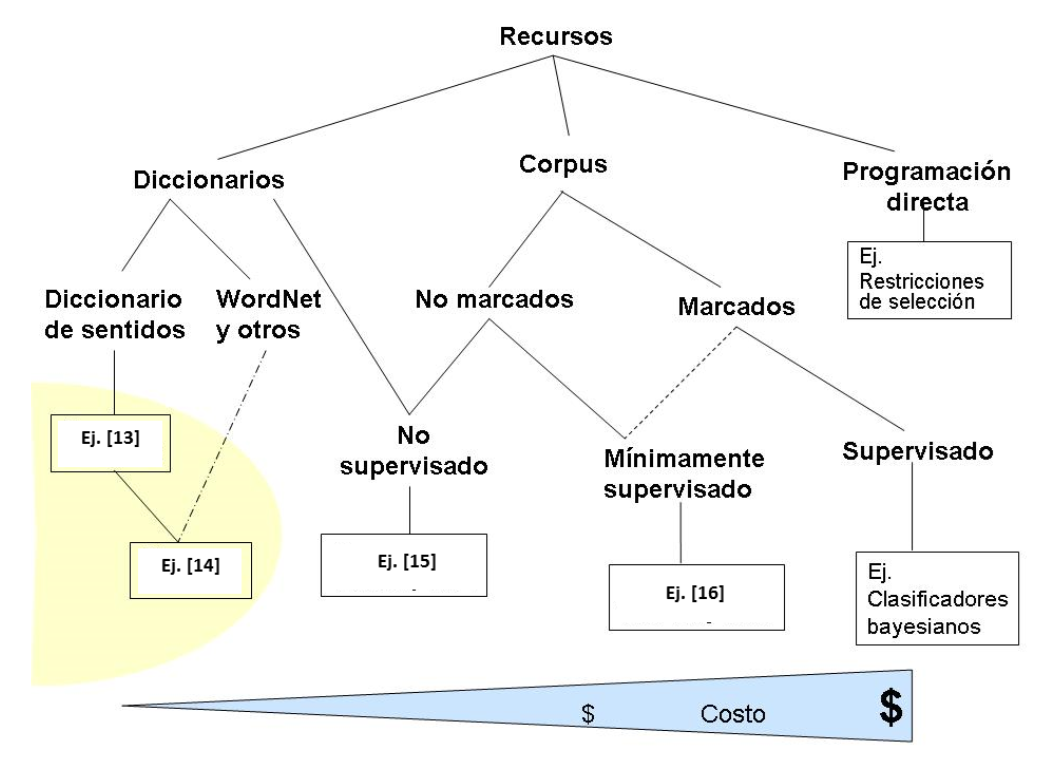
\includegraphics[angle=0, width=10cm]{Graficos/desambiguacion_WSD}
	  \caption{Clasificación de los métodos para WSD de acuerdo a los recursos que utilizan [1].}
    \end{center}
	\end{figure}

\section{Clasificación de sistemas en WSD}
\subsection{Métodos basados en conocimiento}
En esta categoría encontramos diferentes algoritmos para la etiquetación automática de sentidos. Normalmente, el rendimiento de estos métodos basados en conocimiento, es menor en comparación con los métodos basados en corpus. Pero con la salvedad de que los métodos basados en conocimiento tienen una amplia cobertura ya que pueden aplicarse a cualquier tipo de texto en comparación con los basados en corpus que sólo se pueden aplicar a aquellas palabras de las que se dispone de corpus anotados. A continuación, vamos a enumerar diferentes técnicas utilizadas por los métodos basados en conocimiento, aplicables sobre cualquier base de conocimiento léxica que defina sentidos de palabras y relaciones entre ellas. La base de conocimiento léxica más utilizada es WordNet (Miller (1995)). Vamos a describir 4 tipos diferentes de métodos basados en conocimiento:

\begin{itemize}
  \item Algoritmo de Lesk
  \item Similitud semántica
  \item Preferencias de selección
  \item Métodos Heurísticos
\end{itemize}

\subsubsection{Algoritmo de Lesk}
El algoritmo de Lesk [2] es uno de los primeros algoritmos exitosos usados en la desambiguación de sentidos de palabras. Este algoritmo se basa en dos puntos principales: un algoritmo de optimización para WSD y una medida de similitud para las definiciones de los sentidos.
El primer punto es acerca de desambiguar palabras considerando la coherencia global del texto, esto es, encontrar la combinación de los sentidos que maximice la relación total entre los sentidos de todas las palabras. 
Por ejemplo, para la oración \textit{My father deposits his money in a bank account} y considerando a lo más tres sentidos (véase tabla 1), para cada palabra, la figura 2 muestra la representación gráfica del algoritmo original de Lesk.

  \begin{figure}[h!]
    \begin{center}
    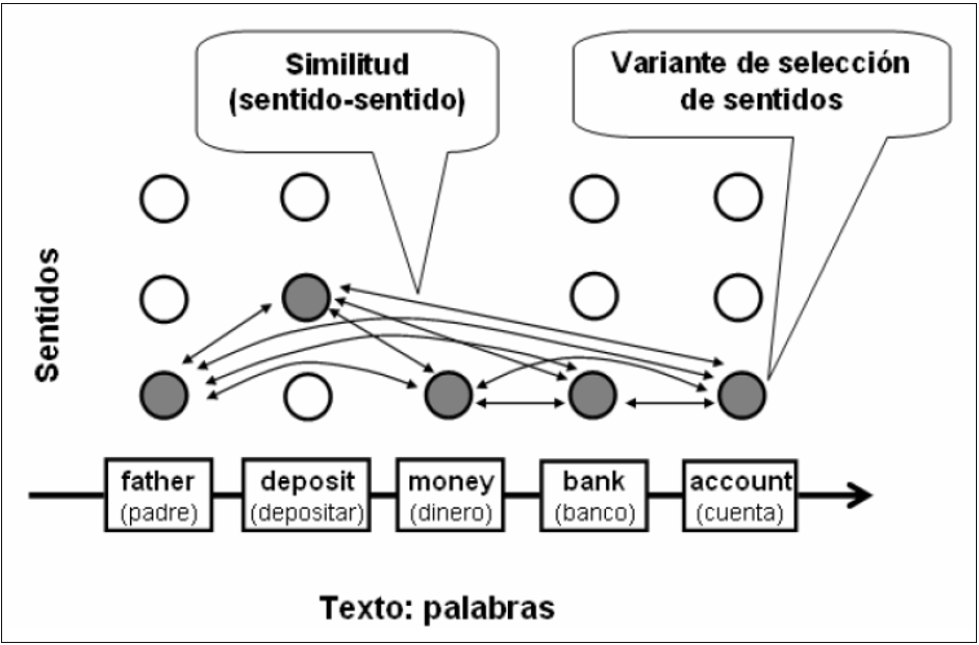
\includegraphics[angle=0, width=10cm]{Graficos/algoritmo_lesk}
    \caption{Representación gráfica del algoritmo original de Lesk [1]}
    \end{center}
  \end{figure}

  Tabla 1. Sentidos de las palabras (máximo tres) obtenidas de WordNet para la oración \textit{“My father deposits his money in a bank account”}.[1]

  \begin{table}[t]
    \centering
    \begin{tabular}{|m{2cm}|m{10cm}|}
    \hline
    % after \\: \hline or \cline{col1-col2} \cline{col3-col4} ...
    Palabra & Sentidos\\
    \hline
    \hline
    Father & 1: a male parent (also used as a term of address to your father); "his father was born in Atlanta". 
    2: `Father' is a term of address for priests in some churches (especially the Roman Catholic Church or the Orthodox Catholic Church); “`Padre' is frequently used in the military”. 
    3: a person who holds an important or distinguished position in some organization; "the tennis fathers ruled in her favor"; "the city fathers endorsed the proposal".\\
    \hline
    Deposit & bf \\
    \hline
    Money & bf \\
    \hline
    Bank & bf \\
    \hline
    Account& bf \\
    \hline
  \end{tabular}
    \caption{Como hacer una tabla}\label{tab:demo}
  \end{table}

\subsubsection{Similitud semántica}
\subsubsection{Preferencias de selección}
\subsubsection{Métodos Heurísticos}
\subsection{Métodos basados en corpus no supervisados}
\subsection{Métodos basados en corpus supervisados}
\subsection{Métodos híbridos}
%La forma como colocar un algoritmo es mediante el
%\verb"\usepackage{algorithmic}" y \verb"{algorithm}" este imprime de
%la siguiente forma:

\bigskip
\begin{algorithm}
\caption{Mapeamiento}\label{mapeadoEVA} processo\_ID(Identificación de flags)\\
Require: Lista de ${1\ldots N}$ que contenga los ID de las clases
correspondientes(provenientes del $FM$).
\begin{algorithmic} [1]
\STATE Generar \emph{lista} a partir de pares correspondientes según
$FM$ \WHILE {SchemaB contenga alguna clase}
\IF{valorASIG(\emph{claseB}) $\geq$ parametro \verb"VAL"}\STATE
\emph{claseB} $\Longleftarrow$ siguiente clase de SchemaB \STATE
\emph{lista} $\Longleftarrow$ agregar los términos de \emph{claseB}
y su correspondiente \emph{claseA} \STATE valor
(\emph{lista$(A_{i},B_{j})$})=\verb"POS"=$1$ \ENDIF \ENDWHILE
\end{algorithmic}
\end{algorithm}

NOTA: Este package no viene incluido por default en el \LaTeX ni con
esta plantilla, pero si es de mucha utilidad, esta disponible en
internet así como muchas otras. Si desean incluir un nuevo
\verb"\usepackage{Nombre_Package}", solo deben agregarla en el
archivo \verb"unsa.cls" en una linea y ya estará disponible.

\begin{table}[h]
  \centering
  \begin{tabular}{|c|c|c|c|c|}
  \hline
  % after \\: \hline or \cline{col1-col2} \cline{col3-col4} ...
  Me & Sem & Lug & Pos & Gen\\
  & Cas & & &\\
  \hline
  \hline
  a & bf & sd & as & hj \\
  a & bf & sdff & fg & ert \\
  a & bf & as & fg & klj \\
  \hline
\end{tabular}
  \caption{Como hacer una tabla}\label{tab:demo}
\end{table}


\begin{figure}
\begin{center}

\includegraphics[angle=45, width=5cm]{Graficos/escuela}
\caption{Logotipo de la EPCC}
\end{center}
\end{figure}

\chapter{Teoría propuesta}
\hrule \bigskip \vspace*{1cm}
%------------------------------------------------------------------------
Cuando queremos definir qué es lenguaje natural, nos hacemos la pregunta ¿Qué surgió primero las reglas gramaticales o el lenguaje? Un lenguaje natural es aquel que ha evolucionado con el tiempo para fines de comunicación humana, como el español o alemán \cite{BROOKSHEAR}.
Estos lenguajes continúan su evolución sin considerar la gramática, cualquier regla se desarrolla después de sucedido el hecho. En contraste, los lenguajes formales están definidos por reglas preestablecidas, y por tanto se rigen con todo rigor a ellas. El lenguaje natural(LN) es el medio que utilizamos de manera cotidiana para establecer nuestra comunicación con las demás personas. El LN ha venido perfeccionándose a partir de la experiencia a tal punto que  puede ser utilizado para analizar situaciones altamente
complejas y razonar muy sutilmente. Los lenguajes naturales tienen un gran poder expresivo y su función y valor como una herramienta para razonamiento. Por otro lado, la sintaxis de un LN puede ser modelada fácilmente por un lenguaje formal, similar a los utilizados en las matemáticas y la lógica.

\section{Arquitectura de un sistema de PLN}

La arquitectura de un sistema de PLN se sustenta en
una definición del LN por niveles: estos son : fonológico, morfológico, sintáctico, semántico, y pragmático.

\begin{description}
\item[Nivel Fonológico:] trata de cómo las palabras se relacionan con los sonidos que representan.
\item[Nivel Morfológico:]  trata de cómo las palabras se construyen a partir de unas unidades de significado más pequeñas llamadas morfemas.
\item[Nivel Sintáctico: ] trata de cómo las palabras pueden unirse para formar  oraciones, fijando el papel estructural que cada palabra juega en la oración y que sintagmas son parte de otros sintagmas.
\item[ Nivel Semántico:] trata del significado de las palabras y de cómo los  significados se unen para dar significado a una oración, también se refiere al  significado independiente del contexto, es decir de la oración aislada.
\item[Nivel Pragmático:]  trata de cómo las oraciones se usan en distintas situaciones y de cómo el uso afecta al significado de las oraciones. Se reconoce un subnivel recursivo: discursivo, que trata de cómo el significado de una oración se ve afectado por las oraciones inmediatamente anteriores.
\end{description}

\section{Problema del procesamiento de lenguaje natural}

En \cite{Arquitectura} nos comenta  la principal dificultad en los procesos de recuperación
de información mediante lenguajes formales no es de índole técnica sino psicológica: entender cuál es la necesidad real del usuario, cual es la correcta formulación de su pregunta o necesidad. La dirección más prometedora de resolver este problema es el uso de lenguaje natural. Sin embargo, uno de los grandes problemas del PLN se produce cuando una expresión en LN posee más de una interpretación, es decir, cuando en el lenguaje de destino se le pueden asignar dos o más expresiones distintas. Este problema de la ambigüedad se presenta en todos los niveles del lenguaje, sin excepción. Ejemplo:
“Hay alguien en la puerta, que te quiere hablar”
“ Hay alguien, en la puerta que te quiere hablar”
No está claro, si el predicado “te quiere hablar” se adjudica a “alguien” o a “la puerta”, sabemos que la puertas no hablan, por tanto deducimos que es a alguien. Pero
esto no lo puede deducir la máquina, a no ser que esté enterada de lo que hacen o no hacen las puertas. En apariencia este problema es demasiado sencillo, pero en realidad, es uno de los más complicados y que más complicaciones ha dado para que el PLN pueda desarrollarse por completo, ya que al presentarse en todos los niveles del lenguaje, se tienen que desarrollar programas (lenguaje formal) para solucionarlos en cada caso.

El error es ta claro por eso tratamos de demostrar La informática ha evolucionado desde sus inicios, considerando siempre aspectos del comportamiento del usuario en relación con el tratamiento de la información. Es por eso que ha incorporado textos, imágenes y
sonido a las estaciones de trabajos actuales, al tiempo que éstos aumentan su capacidad.

La informática ha evolucionado desde sus inicios, considerando siempre aspectos del comportamiento del usuario en relación con el tratamiento de la información. Es por eso que ha incorporado textos, imágenes y sonido a las estaciones de trabajos actuales, al tiempo que éstos aumentan su capacidad.

Los sistemas multimedia incluyen:
\begin{itemize}
  \item Entornos visuales
  \item Autopistas de información
  \item Ratón
  \item Programación interactiva
  \item Realidad Virtual
  \item Hipertexto
  \item Sonido
\end{itemize}

La multimedia combina el hipertexto con el sonido. Estas uniones de imágenes, texto y sonidos necesitan una filosofía del conocimiento que fundamente su función interna dentro de la comunicación de conocimientos. Existe una comunicación sistema-usuario que se da a través de un lenguaje natural que se ve afectado grandemente por el conocimiento que un interlocutor tiene del otro y por el contexto o entorno donde el diálogo tiene lugar.


En \cite{Arquitectura} hace referencia al conocimiento semántico dando como definición que la información sobre el significado se da a las diversas construcciones sintácticas y de cómo esos significados se combina para formar el significado de las oraciones.


\chapter{Experimentación}
\hrule \bigskip \vspace*{1cm}
%------------------------------------------------------------------------

En este capítulo describiremos la aplicación de una de las técnicas de clasificación como parte del aprendizaje supervisado basado en corpus. Para ello se han tomado dos fuentes de entrenamiento, una de elaboración propia (en español) y otra fuente disponible en el sitio \emph{Web} kaggle.com (en inglés).

La fuente de elaboración propia contiene porciones extraídas del resumen de usuarios que exponen su perfil profesional en un sitio especializado como LinkedIn. Para la fase de entrenamiento se espera clasificar perfiles que coinciden con el perfil de "Analista Programador" y diferenciarlos de otros como por ejemplo "Analista Funcional" o "Analista de Planeamiento", entre otros.

Con respecto a la fuente descargada en inglés, ésta contiene tweets con mensajes ofensivos y no ofensivos. Al estar en un sitio público, ésta contiene mayor cantidad de datos de entrenamiento, lo cual permite lograr un mejor entrenamiento durante la fase de aprendizaje.

\section{Procedimiento}

Como algoritmo de clasificación se utilizó kNN (k-Nearest Neighbors). El procedimiento aplicado para la clasificación y pronóstico de textos mostrado en la figura \ref{fig:experimentacion} inicia con el entrenamiento del modelo, para ello se requiere de una fuente de datos previamente etiquetada. En la fase de predicción, se prueba el modelo con un conjunto de textos distinto al inicial (conjunto de prueba), el cual también está etiquetado para su verificación posterior.

Finalmente el resultado (conjunto de predicciones) se compara con el valor esperado del conjunto de prueba para el análisis respectivo.


\begin{figure}[h!]
	\begin{center}
	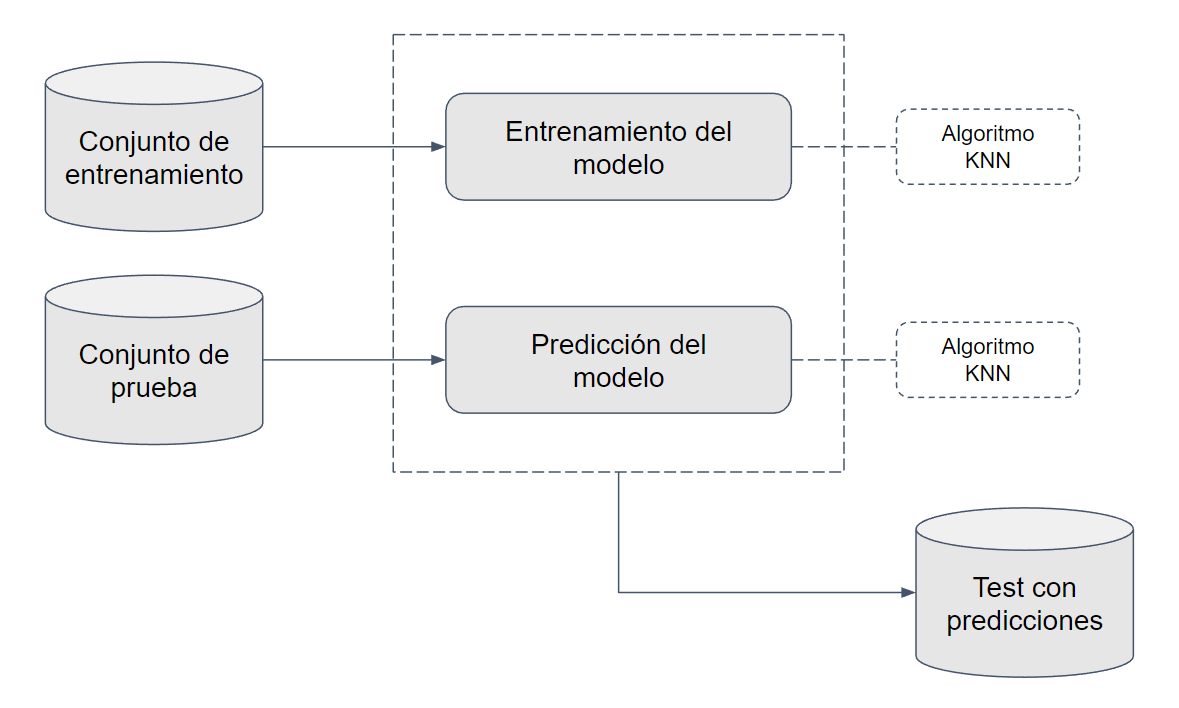
\includegraphics[angle=0,width=9.5cm]{Graficos/experimentacion1}
	\caption{Procedimiento aplicado para del método de clasificación.}
	\label{fig:experimentacion}
  \end{center}
\end{figure}

\section{Tratamiento del texto}

\subsection{Bolsa de palabras}

En esta primera fase, el texto de entrada pasa por un proceso inicial de preparación (tokenización), luego se procede a extraer características del texto (diccionario) y la frecuencia de cada una. Finalmente el diccionario de palabras se transforma en un vector de características para cada entrada (frase o tweet). La figura \ref{fig:bolsa} muestra este proceso con los resultados de forma visual.

Durante la tokenización, se extraen símbolos y carácteres no reconocibles. En el caso de los tweets, hay mayor cantidad de textos no reconocibles al provenir de una fuente de mensajería informal (se utilizan abreviaciones, emojis, o repeticiones de algunas letras, por ejemplo: 'awwwwww', 'noooo', 'lol', 'xD').

Teniendo el texto libre de símbolos extraños, se procede a extraer un diccionario de palabras con su respectiva frecuencia, tal como se muestra en la segunda parte de la figura \ref{fig:bolsa}. Este diccionario sirve para convertir cada texto de entrada en un vector de características, donde cada elemento del mismo representa la cantidad de veces que aparece una palabra determinada en el texto. Este vector es de N dimensiones, contiene muchos ceros (palabras que no aparecen en el texto), por lo cual es conveniente aplicar algún método de reducción de dimensionalidad.

\begin{figure}[h!]
	\begin{center}
	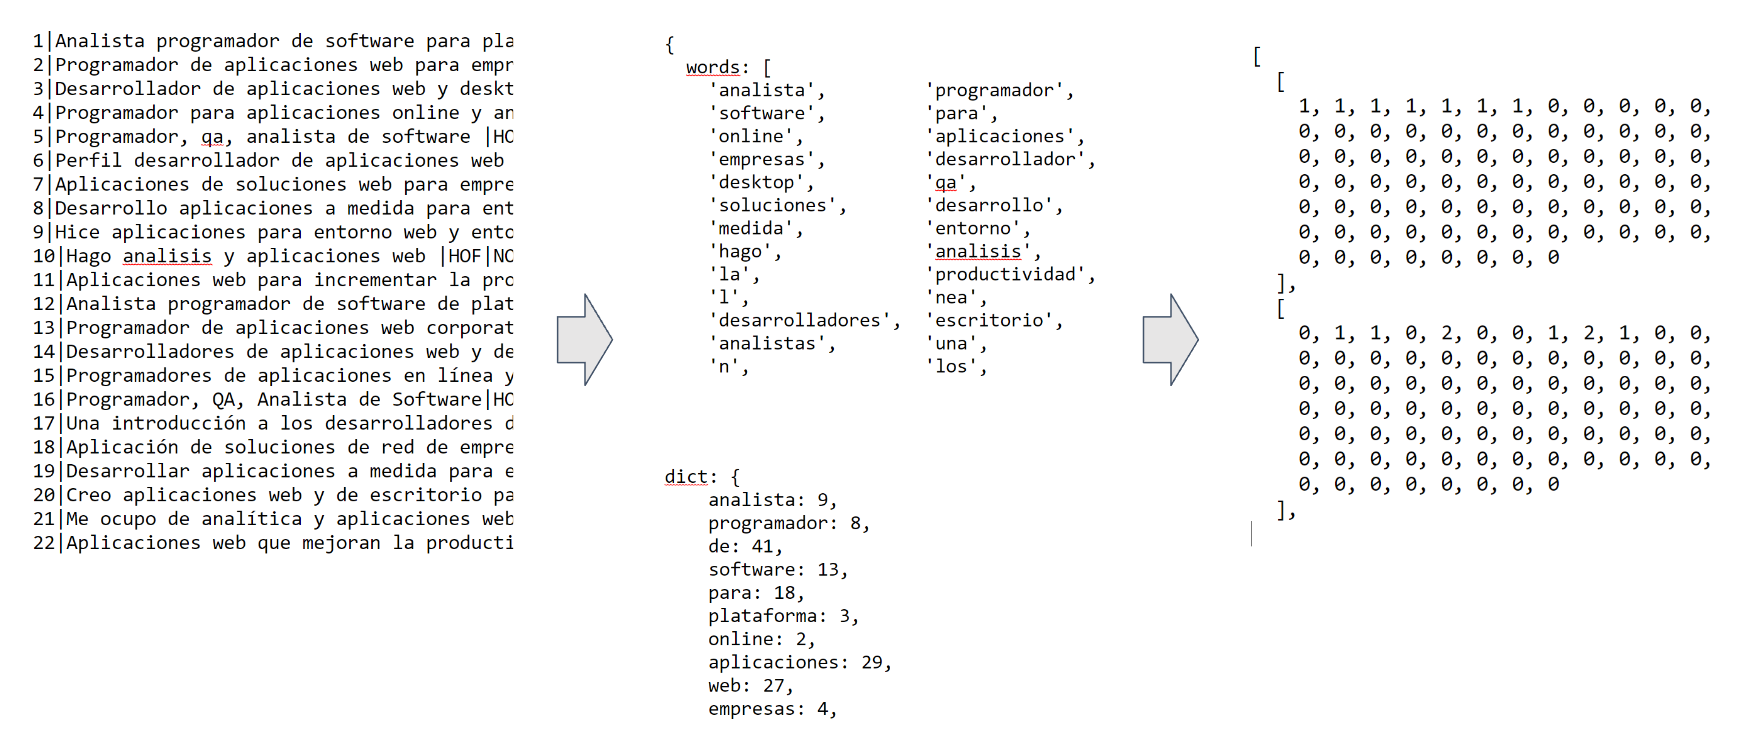
\includegraphics[angle=0,width=9.5cm]{Graficos/bolsa_palabras}
	\caption{Tratamiento del texto al aplicar la bolsa de palabras.}
	\label{fig:bolsa}
  \end{center}
\end{figure}

\subsection{Reducción de dimensiones}

El vector de características que se obtiene luego de aplicar la Bolsa de Palabras, es de N dimensiones, dependiendo de qué tan grande es el diccionario generado. Cuanto más grande sea la variedad de palabras mayor será el tamaño del diccionario y en consecuencia el tamaño del vector generado.

Aplicar un algoritmo de clasificación sobre este vector de N dimensiones no es aconsejable, por el procesamiento alto que conlleva trabajar de N dimensiones; en ese sentido, es necesario reducir la dimensionalidad de dicho vector.

Para este experimento, se aplica el algoritmo MDS (\emph{Multidimensional Scaling}) cuyo detalle se explicó en la sección \ref{mds}. Para efectos prácticos, se aplicó una reducción a 2 dimensiones. La figura \ref{fig:mds} muestra el resultado luego de aplicar el algoritmo al vector N-dimensional resultado de la bolsa de palabras.

\begin{figure}[h!]
	\begin{center}
	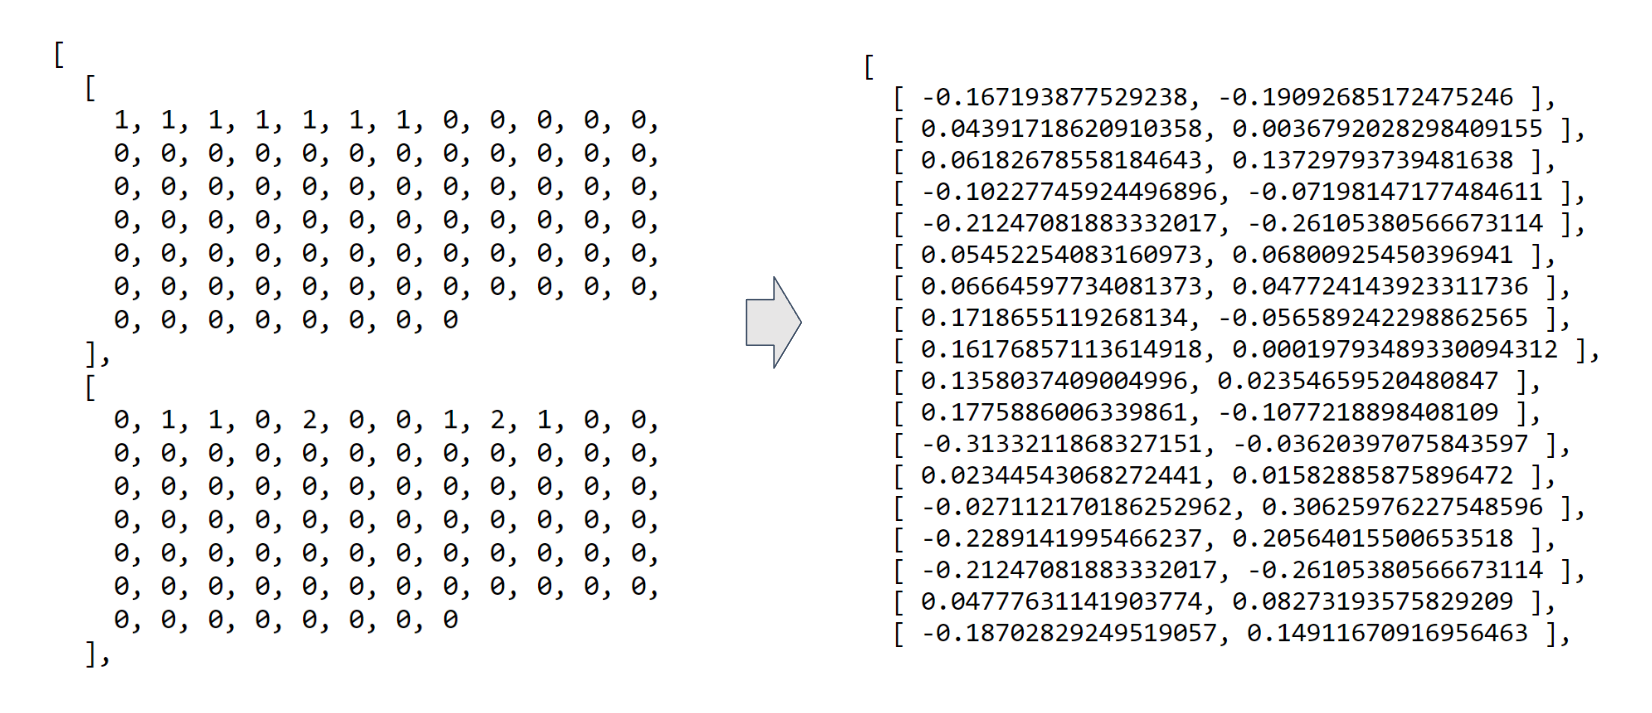
\includegraphics[angle=0,width=9.5cm]{Graficos/mds}
	\caption{Reducción de dimensiones aplicando el algoritmo MDS.}
	\label{fig:mds}
  \end{center}
\end{figure}

\subsection{Reducción de dimensiones}

El vector de características que se obtiene luego de aplicar la Bolsa de Palabras, es de N dimensiones, dependiendo de qué tan grande es el diccionario generado. Cuanto más grande sea la variedad de palabras mayor será el tamaño del diccionario y en consecuencia el tamaño del vector generado.

Aplicar un algoritmo de clasificación sobre este vector de N dimensiones no es aconsejable, por el procesamiento alto que conlleva trabajar de N dimensiones; en ese sentido, es necesario reducir la dimensionalidad de dicho vector.

Para este experimento, se aplica el algoritmo MDS (\emph{Multidimensional Scaling}) cuyo detalle se explicó en la sección \ref{mds}. Para efectos prácticos, se aplicó una reducción a 2 dimensiones. La figura \ref{fig:mds} muestra el resultado luego de aplicar el algoritmo al vector N-dimensional resultado de la bolsa de palabras.

\begin{figure}[h!]
	\begin{center}
	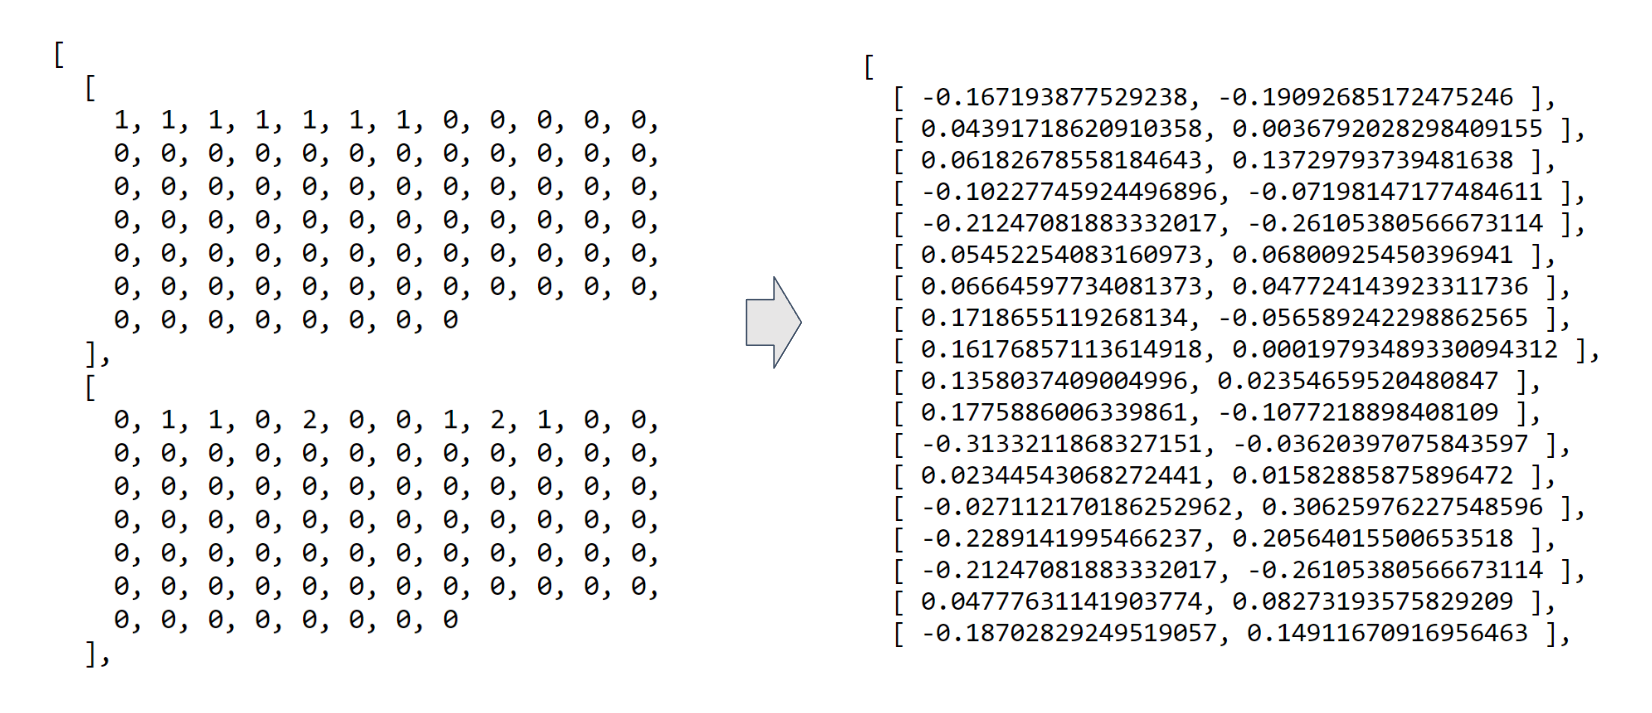
\includegraphics[angle=0,width=9.5cm]{Graficos/mds}
	\caption{Reducción de dimensiones aplicando el algoritmo MDS.}
	\label{fig:mds}
  \end{center}
\end{figure}

\subsection{Clasificación y entrenamiento}

Como se mencionó anteriormente, el algoritmo de clasificación utilizado es el \emph{kNN}. Su implementación está basada en una estructura \emph{KD Tree} y se escogió un valor de $k = 7$ para el experimento. De esta forma se seleccionarán los 7 vecinos más cercanos para clasificar los nuevos mensajes.

La figura \ref{fig:knn_train} la distribución de puntos en 2D, diferenciando las clases en color rojo y verde. Para el conjuntos de entrenamiento relacionados a tweets, en inglés, se muestran en color verde los tweets clasificados como no ofensivos y en rojo los ofensivos. Para el conjunto de entrenamiento relacionados a resúmenes de perfil profesional, en verde los textos relacionados a un perfil de Analista Programador o Desarrolladores, y en rojo los que están relacionados a otro perfil.

Los resultados se muestran en la figura \ref{fig:knn_train_results}. La aplicación del algoritmo sobre el conjunto de prueba es un conjunto de vectores con la posición final de cada punto y la clasificación respectiva, hecha en base a los k vecinos más cercanos ($k = 7$);

Finalmente, cuando se pretende evaluar un mensaje nuevo, se muestra un punto de color negro y el resultado de la clasificación.

\begin{figure}[h!]
	\begin{center}
	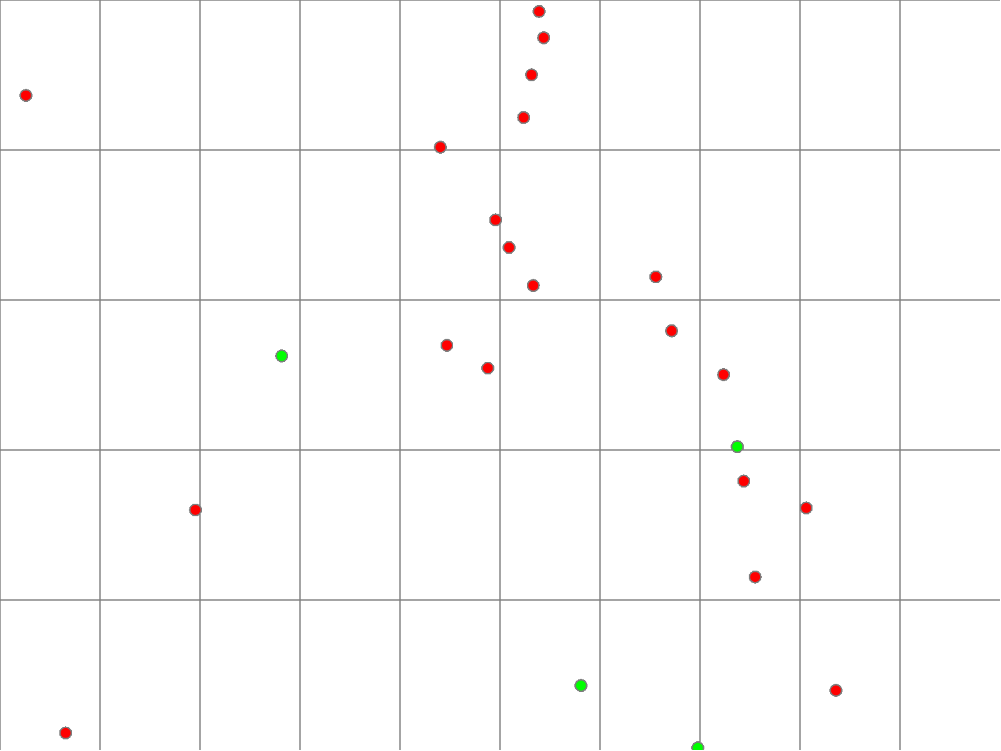
\includegraphics[angle=0,width=9.5cm]{Graficos/knn_train}
	\caption{Clasificación de mensajes de entrenamiento.}
	\label{fig:knn_train}
  \end{center}
\end{figure}


\begin{figure}[h!]
	\begin{center}
	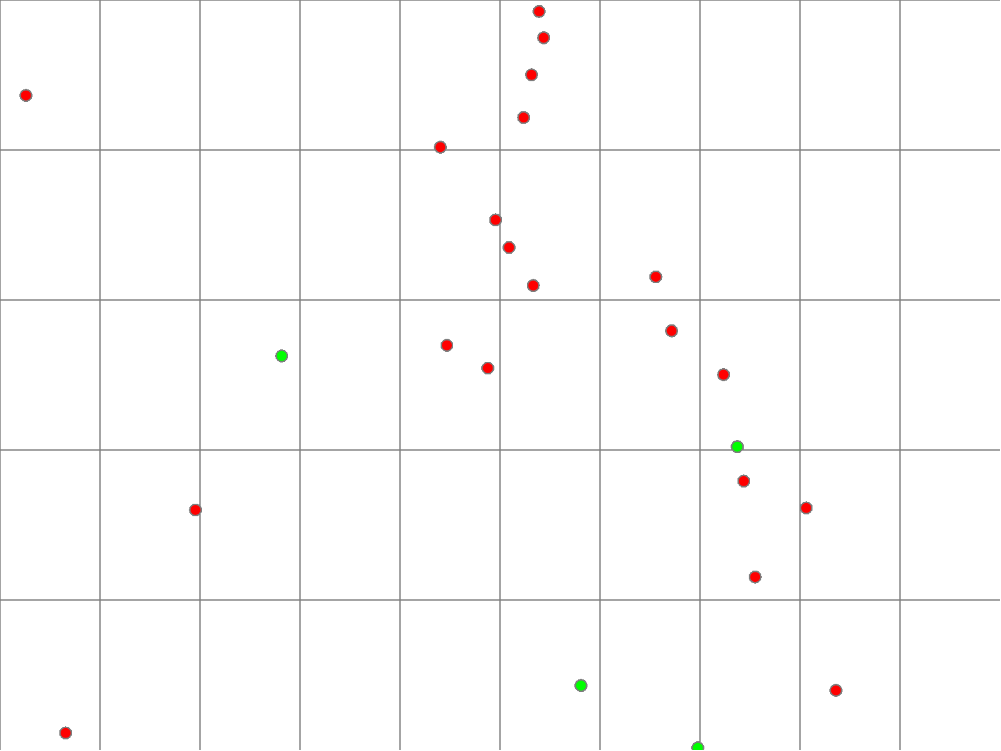
\includegraphics[angle=0,width=9.5cm]{Graficos/knn_train_results}
	\caption{Clasificación de mensajes de entrenamiento.}
	\label{fig:knn_train_results}
  \end{center}
\end{figure}


\section{Resultados}

En la figura  \ref{fig:Comparacion1}   en la parte (A) mostramos los puntos en negro a ser clasificados por nuestro algoritmo, en la parte (B) mostramos el resultado luego de la clasificación.


\begin{figure}[h!]
	\begin{center}
	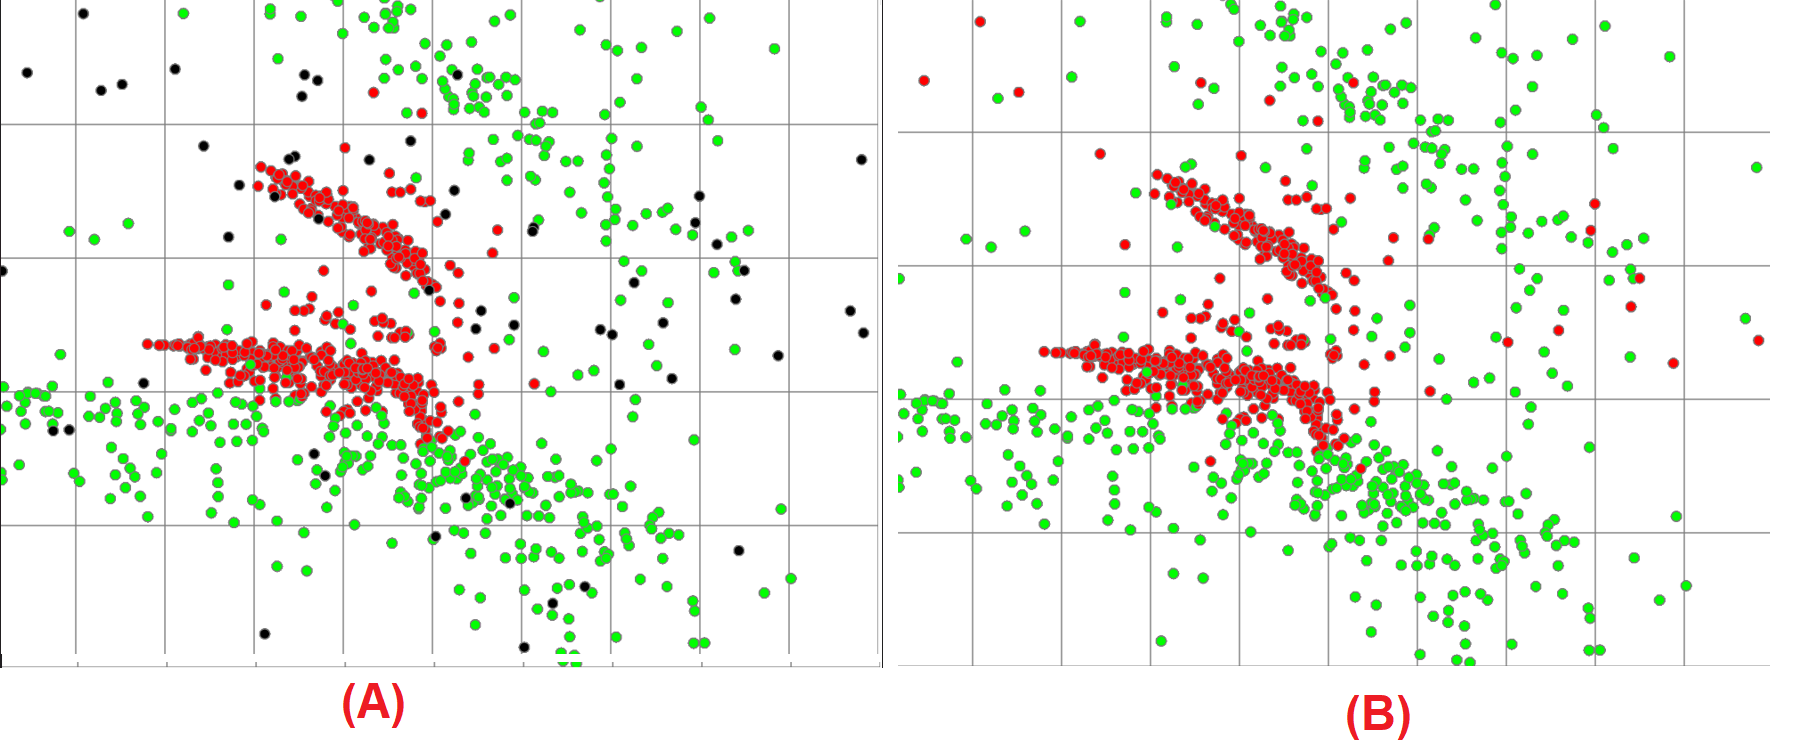
\includegraphics[ width=15cm]{Graficos/Comparacion1}
	\caption{Resultado después de la prueba  }
	\label{fig:knn_experimento}
  \end{center}
\end{figure}

\chapter{Resultados}
\hrule \bigskip \vspace*{1cm}
%------------------------------------------------------------------------
\section{Conclusiones}
\begin{itemize}
  \item El lenguaje natural (LN) nos permite el designar las cosas actuales y razonar acerca de ellas, fue desarrollado y organizado a partir de la experiencia humana y puede ser utilizado para analizar situaciones altamente complejas y razonar muy sutilmente.
 \item  Los lenguajes de programación (LP) son un tipo muy limitado de lenguaje natural, orientados básicamente a la manipulación de datos e información discreta, pero no son suficientes para la comunicación integral que incluya la totalidad de los aspectos semánticos y pragmáticos.
 \item  El procesamiento de lenguaje natural (PLN) consiste en la utilización de un lenguaje natural para comunicarnos con la computadora, debiendo esta entender las oraciones que le sean proporcionadas. El uso de estos lenguajes naturales facilita el desarrollo de programas que realicen tareas relacionadas con el lenguaje o bien, desarrollar modelos que ayuden a comprender los mecanismos humanos relacionados con el lenguaje. Los lexicones son una parte importante del procesamiento de lenguaje natural y debe contener información fonológica, morfológica, sintáctica, semántica y pragmática, pero además esta información debe ser estructurada de forma que permita su reutilización para diversas tareas.
 \item  El lexicón también tiene que incluir otros tipos de información que considere aspectos de orden idiosincrática, de pronunciación, y toda información que no se puede derivar del significado de las palabras o de su forma morfológica.
\end{itemize}

\section{Contribuciones}

Con todo lo que has investigado, propuesto y/o desarrollado que haz
conseguido obtener para cooperar con la solución del problema.

\section{Trabajo futuro}

A partir del conocimiento generado en disciplinas como la informatica y la lingüística computacional, se están desarrollando sistemas para la confección de resúmenes y la indización automática. Este tipo de investigaciones se lleva practicando desde hace tiempo, y se comienza a recoger los frutos de años de inspección, por lo que se debe permanecer atentos a su evolución. El procesamiento del lenguaje natural es una labor
compleja, no exento de dificultad para los lingüísticas que deben adquirir la instrumentación de los informáticos, y para los informáticos, ya que deben hacer suyos
conocimientos lingüísticos.

\myappendix{Apendice}
\begin{singlespace}
\bibliographystyle{apalike}%plain
\mybibliography{biblio}
\end{singlespace}
\end{document}%%%%%%%%--------------------------------------------------------
